\hypersetup{colorlinks=true, linkcolor=blue, citecolor=red}

\chapter{Dataset analysis} \label{chap:dataset_analysis}

    In this chapter, the dataset used in this thesis is analyzed. The data collection methodology is described, along with a recording setup. Data structure and attributes are presented, along with patient's characteristics. Finally, data processing steps are described.

    \section{Data collection methodology}
        
        Data used in this thesis is collected at Waterford Hospital in Ireland as part of a Fear of Falling study conducted on a group of 22 elderly individuals. Following a recording setup a Microsoft Kinect is used to record movements performed. 

        \subsection{Microsoft kinect}

            The first generation of Kinect sensor, Kinect V1 in Figure \ref{fig:kinect_sensor}, is a motion sensing input device developed by Microsoft and first released in 2010 for game consoles and Microsoft Windows PCs \cite{xu_validity_2015}. A new version of a Kinect sensor, Kinect V2, was released in 2014, with improved hardware and software \cite{cruz_kinect_2012}. 

            \begin{figure}[H]
                \centering
                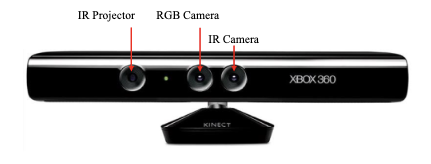
\includegraphics[width=0.6\textwidth]{./resources/images/kinect/kinect.png}
                \caption{Microsoft Kinect Sensor.}
                \label{fig:kinect_sensor}
            \end{figure}

                    \subsubsection{Kinect sensor} 

                        Kinect Sensor is a horizontal bar connected to a small base with a motorized pivot and is designed to be positioned lengthwise above or below a video display. The device features a color camera, an infrared (IR) emitter, an IR depth sensor, an engine for tilting, a microphone array, and an LED light \cite{abbasi_motion_2021}. The sensor is capable of sending three types of data: color images, 3D depth images, and bone information corresponding to a 3D imaging field \cite{zheng_cg-recognizer_2022}\cite{acis_classification_2023}. Along with its open-source libraries, the Kinect system has helped to develop a wide range of applications in the fields of computer vision, robotics, and human-computer interaction. This is because Kinect offers a cost-effective and broadly accessible method for capturing 3D human motion data, with the advantage of allowing users to interact with the system without a need for any physical devices \cite{gowing_kinect_2014}.

                
                        \begin{figure}[H]
                            \centering
                            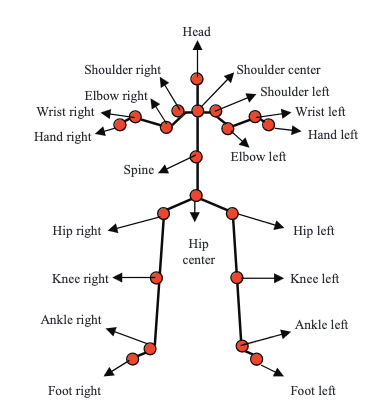
\includegraphics[width=0.6\textwidth]{./resources/images/kinect/joints.png}
                            \caption{Skeletal joints recognized by a Microsoft Kinect sensor \cite{jais_review_2015}.}
                            \label{fig:kinect_sensor_v2}
                        \end{figure}

                    \subsubsection{PyKinect2}
                        PyKinect2 is a Python library for Microsoft's Kinect V2 sensor. It provides a wrapper for Kinect Windows SDK 2.0, which allows for the use of the sensor in Python. Library abstracts complex functionality of the hardware into an easy-to-use API. Key features include:
                        \begin{itemize}
                            \item \textbf{Skeletal tracking}: detects and tracks human bodies, providing joint positions and orientations.
                            \item \textbf{Color, depth, and infrared streams}: Accesses raw sensor streams for visual processing or analysis.
                            \item \textbf{Coordinate mapping}: translates between different spatial representations. Such as mapping skeletal joints to color or depth images for overlay visualization.
                        \end{itemize}
                        PyKinect2 library is a great bridge between Kinect sensor and Python programming language, allowing for the use of the sensor in a variety of applications \cite{GitHubKinectPyKinect2}.
               
                        \newpage
                        
        \subsection{Recording setup}

                    The patient's data recording setup illustrated in Figure \ref{fig:kinect_setup} consists of consumer-level hardware (a laptop, a Kinect V2 depth camera, an external webcam, and a smartphone) and a dedicated application developed within the project. 
                    Once launched, an operator can display a sample stimulus on an external monitor to show target movements to patients (\textit{1. Stimulus playback}) so they can repeat (\textit{2. patient performs movement}) them by selecting one of them from a list in the application.
                    Then, by pressing the "\textit{record}" button (\textit{3. record/analyze skeleton + RGB + accelerometer}), recording of the patient's full body movement can be started. 
                    The application stores recorded patient's movement files in a separate folder, naming them based on their patient ID, movement ID, and repetition ID.

                    \begin{figure}[H]
                        \centering
                        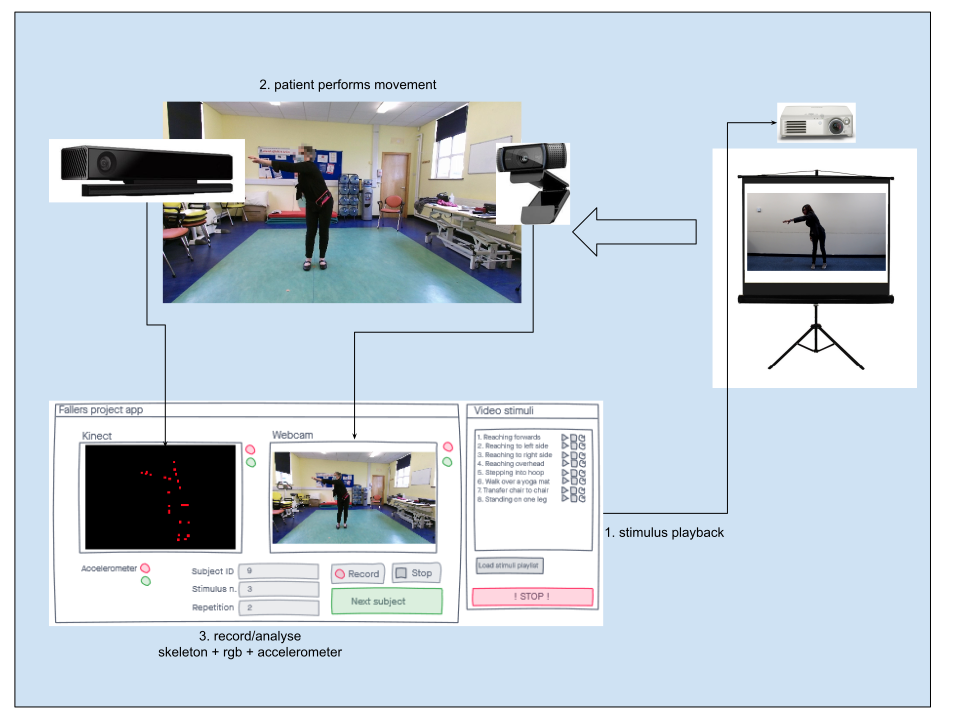
\includegraphics[width=0.9\textwidth]{./resources/images/kinect/setup.png}
                        \caption{Setup used at Waterford Hospital for data collection.}
                        \label{fig:kinect_setup}
                    \end{figure}

                    Full body capture mainly relies on the PyKinect library \cite{GitHubKinectPyKinect2}, which provides functions for getting the patient's body segment's position and rotation 25 times per second. The application gets the data and stores it as a multi-dimensional time series (one per body segment and coordinate type) in CSV files like the one displayed in Figure \ref{fig:csv_structure}.
                    \newpage
                    \begin{figure}[H]
                        \centering
                        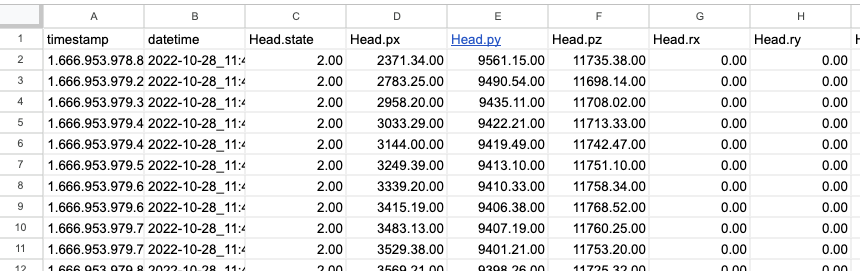
\includegraphics[width=1.0\textwidth]{./resources/images/other/data.png}
                        \caption{Example of a CSV file containing Kinect skeleton data.}
                        \label{fig:csv_structure}
                    \end{figure}

                    The accelerometer is captured via a smartphone running an app streaming 3D gyroscope data at 50 frames per second. Again, the application on the computer stores it as a multi-dimensional time series (one per rotation axis). Communication between smartphone and computer is based on a wireless network and Open Sound Control (OSC) protocol \cite{wright_open_nodate}.
    
    \section{Data structure and attributes}
            
            Data used in this thesis consists of a series of CSV files, each containing 3D coordinates of the joints of a patient performing a movement. Total number of CSV files is \textbf{637}. In Figure \ref{fig:dataset_files} distribution of the CSV files between the movements is presented with a median of \textbf{68} files per movement.

            \begin{figure}[H]
                \centering 
                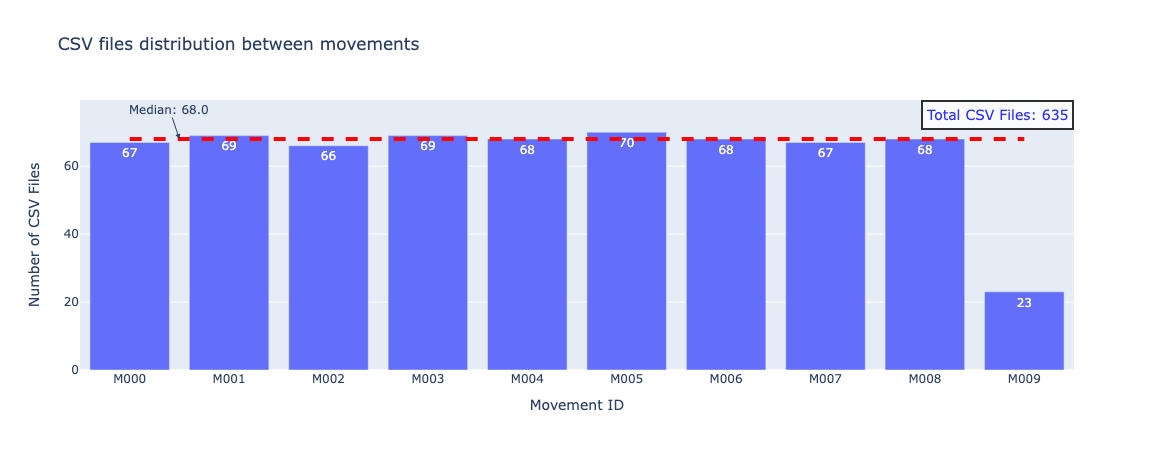
\includegraphics[width=1.0\textwidth]{./resources/plots/patients/csv_files.png}
                \caption{CSV files distribution between movements. \textit{M009} is the only movement with less than 68 files due to it not being performed multiple times by the patients.}
                \label{fig:dataset_files}
            \end{figure}
        
            The dataset is organized in a directory structure. Each patient has a folder named with their ID (\textit{Patient-ID}) and inside there are 10 folders for each movement, named with the movement ID (\textit{M-XXX}). For every movement folder, there is a folder for each repetition of the movement, named with a repetition ID (\textit{R-XXX}). Inside each repetition folder, there is a CSV file that contains Kinect skeleton data. In Figure \ref{fig:directory-structure} an example of a directory structure is displayed. \\
            
            \begin{figure}[htbp]
                \centering
                \begin{forest}
                for tree={
                folder,
                grow'=0,
                fit=band,
                }
                [Patients
                    [Patient-1
                        [M000
                            [R000
                                [FILE.CSV]
                            ]
                            [R001]
                            [R002]
                        ]
                    ]
                ]
                \end{forest}
                \caption{Directory structure example using first patient and first movement in the dataset. }
                \label{fig:directory-structure}
            \end{figure}

            a CSV file is organized as a series of columns, each column representing a joint in Table \ref{tab:joints_recorded} that a Kinect sensor records. Each joint is represented by 7 columns, one for each position and rotation coordinate (x, y, z) and one for the state (used to indicate if the joint is tracked or not). Besides joints columns, there are 2 columns for timestamp and datetime of the recording.
            
            \begin{table}[H]
                \centering
                \begin{tabularx}{1.0\textwidth}{XXXX} 
                    \toprule
                    \multicolumn{4}{c}{\textbf{Joints}} \\ 
                    \midrule
                    AnkleLeft & AnkleRight & ElbowLeft & ElbowRight \\
                    FootLeft & FootRight & HandLeft & HandRight \\ 
                    HandTipLeft & HandTipRight & Head & HipLeft \\
                    HipRight & KneeLeft & KneeRight & Neck \\
                    ShoulderLeft & ShoulderRight & SpineBase & SpineMid \\ 
                    SpineShoulder & ThumbLeft & ThumbRight & WristLeft \\
                    WristRight & & & \\
                    \bottomrule
                \end{tabularx}
                \caption{Joints processed with PyKinect2 library.}
                \label{tab:joints_recorded}
            \end{table}

    \section{Patients characteristics}
        Patients that take part in the study are 22 elderly individuals, in Figure \ref{fig:age_distribution} age distribution is presented, with a median age of 67 years. 
        \newpage 
        \begin{figure}[H]
            \centering
            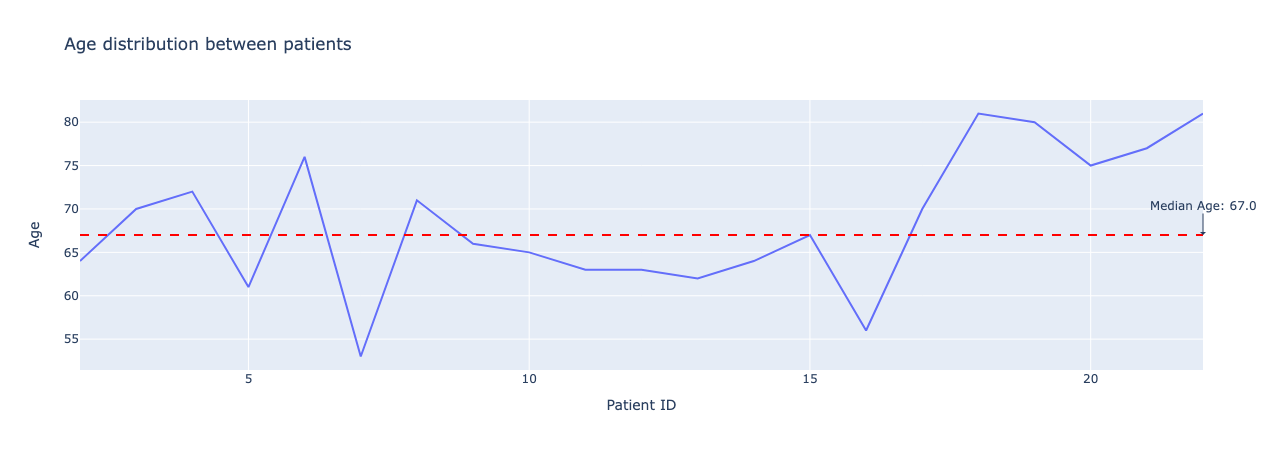
\includegraphics[width=1.0\textwidth]{./resources/plots/patients/age.png}
            \caption{Age distribution of patients.}
            \label{fig:age_distribution}
        \end{figure}

        In Figure \ref{fig:patients_characteristics} patient's characteristics are presented. \textbf{Fear of Falling} is present in \textbf{57\%} of patients, this is a relatively high percentage, due to the study being conducted on a Fear of Falling assessment group. Gender is dominated by \textbf{females} with a \textbf{95\%} of patients, this is also expected since most studies in literature had mostly female patients (>50\%) \cite{mackay_fear_2021}. Education is also presented, with the majority of patients having a \textbf{Secondary} or \textbf{Third Level} education.
        
        \begin{figure}[H]
            \centering
            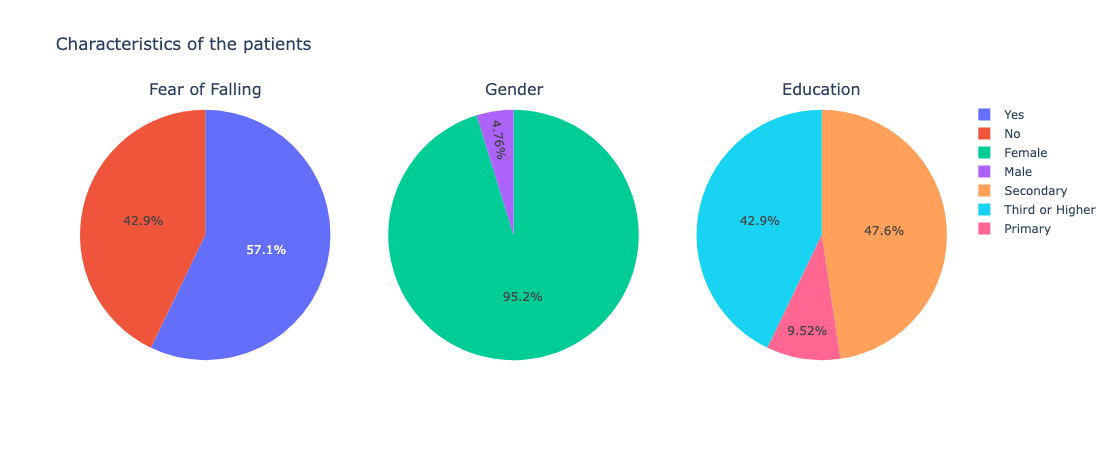
\includegraphics[width=1.0\textwidth]{./resources/plots/patients/chars.png}
            \caption{Characteristics of patients in the study.}
            \label{fig:patients_characteristics}
        \end{figure}

        \subsubsection{What is fear of falling ?}
        
            The definition of \textbf{Fear of Falling} had various interpretations over the years. Initially, it is described as a phobic reaction to standing or walking. However, it is reclassified as a syndrome characterized by the aftermath of a fall. As understanding develops, this fear is seen as a loss of confidence in one's balance ability. It is also further defined as an ongoing concern about falling, which leads to avoidance of performing daily activities. Recently, it has been described as continuous avoidance of activities due to a concern of falling \cite{jung_fear_2008}.
    
    \section{Movements visualization} \label{sec:movements_visualization}
        
        Kinect skeleton data comes as a series of 3D coordinates, which can be visualized in 3D space. In this section, the implementation of movement visualization is presented. It is implemented using Python programming language and Plotly library \cite{plotly}.

        The first step in a visualization process is to identify a set of joints to be used. In this approach, the dataset contains 25 joints but only 16 joints are used and are displayed in Table \ref{tab:joints_select}. 

        \begin{table}[H]
            \centering
            \begin{tabularx}{1.0\textwidth}{XXX}
                \toprule
                \multicolumn{3}{c}{\textbf{Joints}} \\
                \midrule
                Head & Spine Shoulder & Spine Mid \\
                Spine Base & Shoulder Right & Elbow Right \\
                Wrist Right & Shoulder Left & Elbow Left \\
                Wrist Left & Hip Right & Knee Right \\
                Ankle Right & Hip Left & Knee Left \\
                Ankle Left & & \\
                \bottomrule
            \end{tabularx}
            \caption{Selected Kinect joints used for visualization.}
            \label{tab:joints_select}
        \end{table}
        
        Once joints are selected, the next step is to transform the data. In its original state data is organized incorrectly for 3D visualization, and y and z coordinates are inverted. To fix this, the y and z coordinates are swapped. \\

        After the transformation is performed, data is ready to be visualized. Snippet \ref{lst:visualization} shows an implementation of the visualization process, it begins by extracting joint coordinates and their connections, assigning colors and sizes to major joints, and configuring a 3D layout. Animation frames are generated by iteratively capturing snapshots of joint positions and connections over time. These frames are then combined and displayed in an interactive 3D plot, allowing a user to play/stop the animation and rotate the plot to view a movement from different angles.

        \begin{lstlisting}[caption={Code snippet creates connecting lines between joints using their 3D coordinates, enabling visualization of joint movements.}, label={lst:visualization}, language=Python]            
    for index, row in data.iterrows():
        x_values = [row[f"{joint}.px"] for joint in joints]
        y_values = [row[f"{joint}.py"] for joint in joints]
        z_values = [row[f"{joint}.pz"] for joint in joints]
        lines = []
        for connection in connections:
            start, end = connection
            lines.append(go.Scatter3d(
                    x=[row[f"{start}.px"], row[f"{end}.px"]],
                    y=[row[f"{start}.py"], row[f"{end}.py"]],
                    z=[row[f"{start}.pz"], row[f"{end}.pz"]],))
        \end{lstlisting}
        
        \newpage

        In Figure \ref{fig:movements_visualization} a set of movements performed by the patients is presented. The movements are displayed in a 3D plot, with the x, y, and z axes representing plot axes. 

        \begin{figure}[h]
            \begin{subfigure}{.5\textwidth}
                \centering
                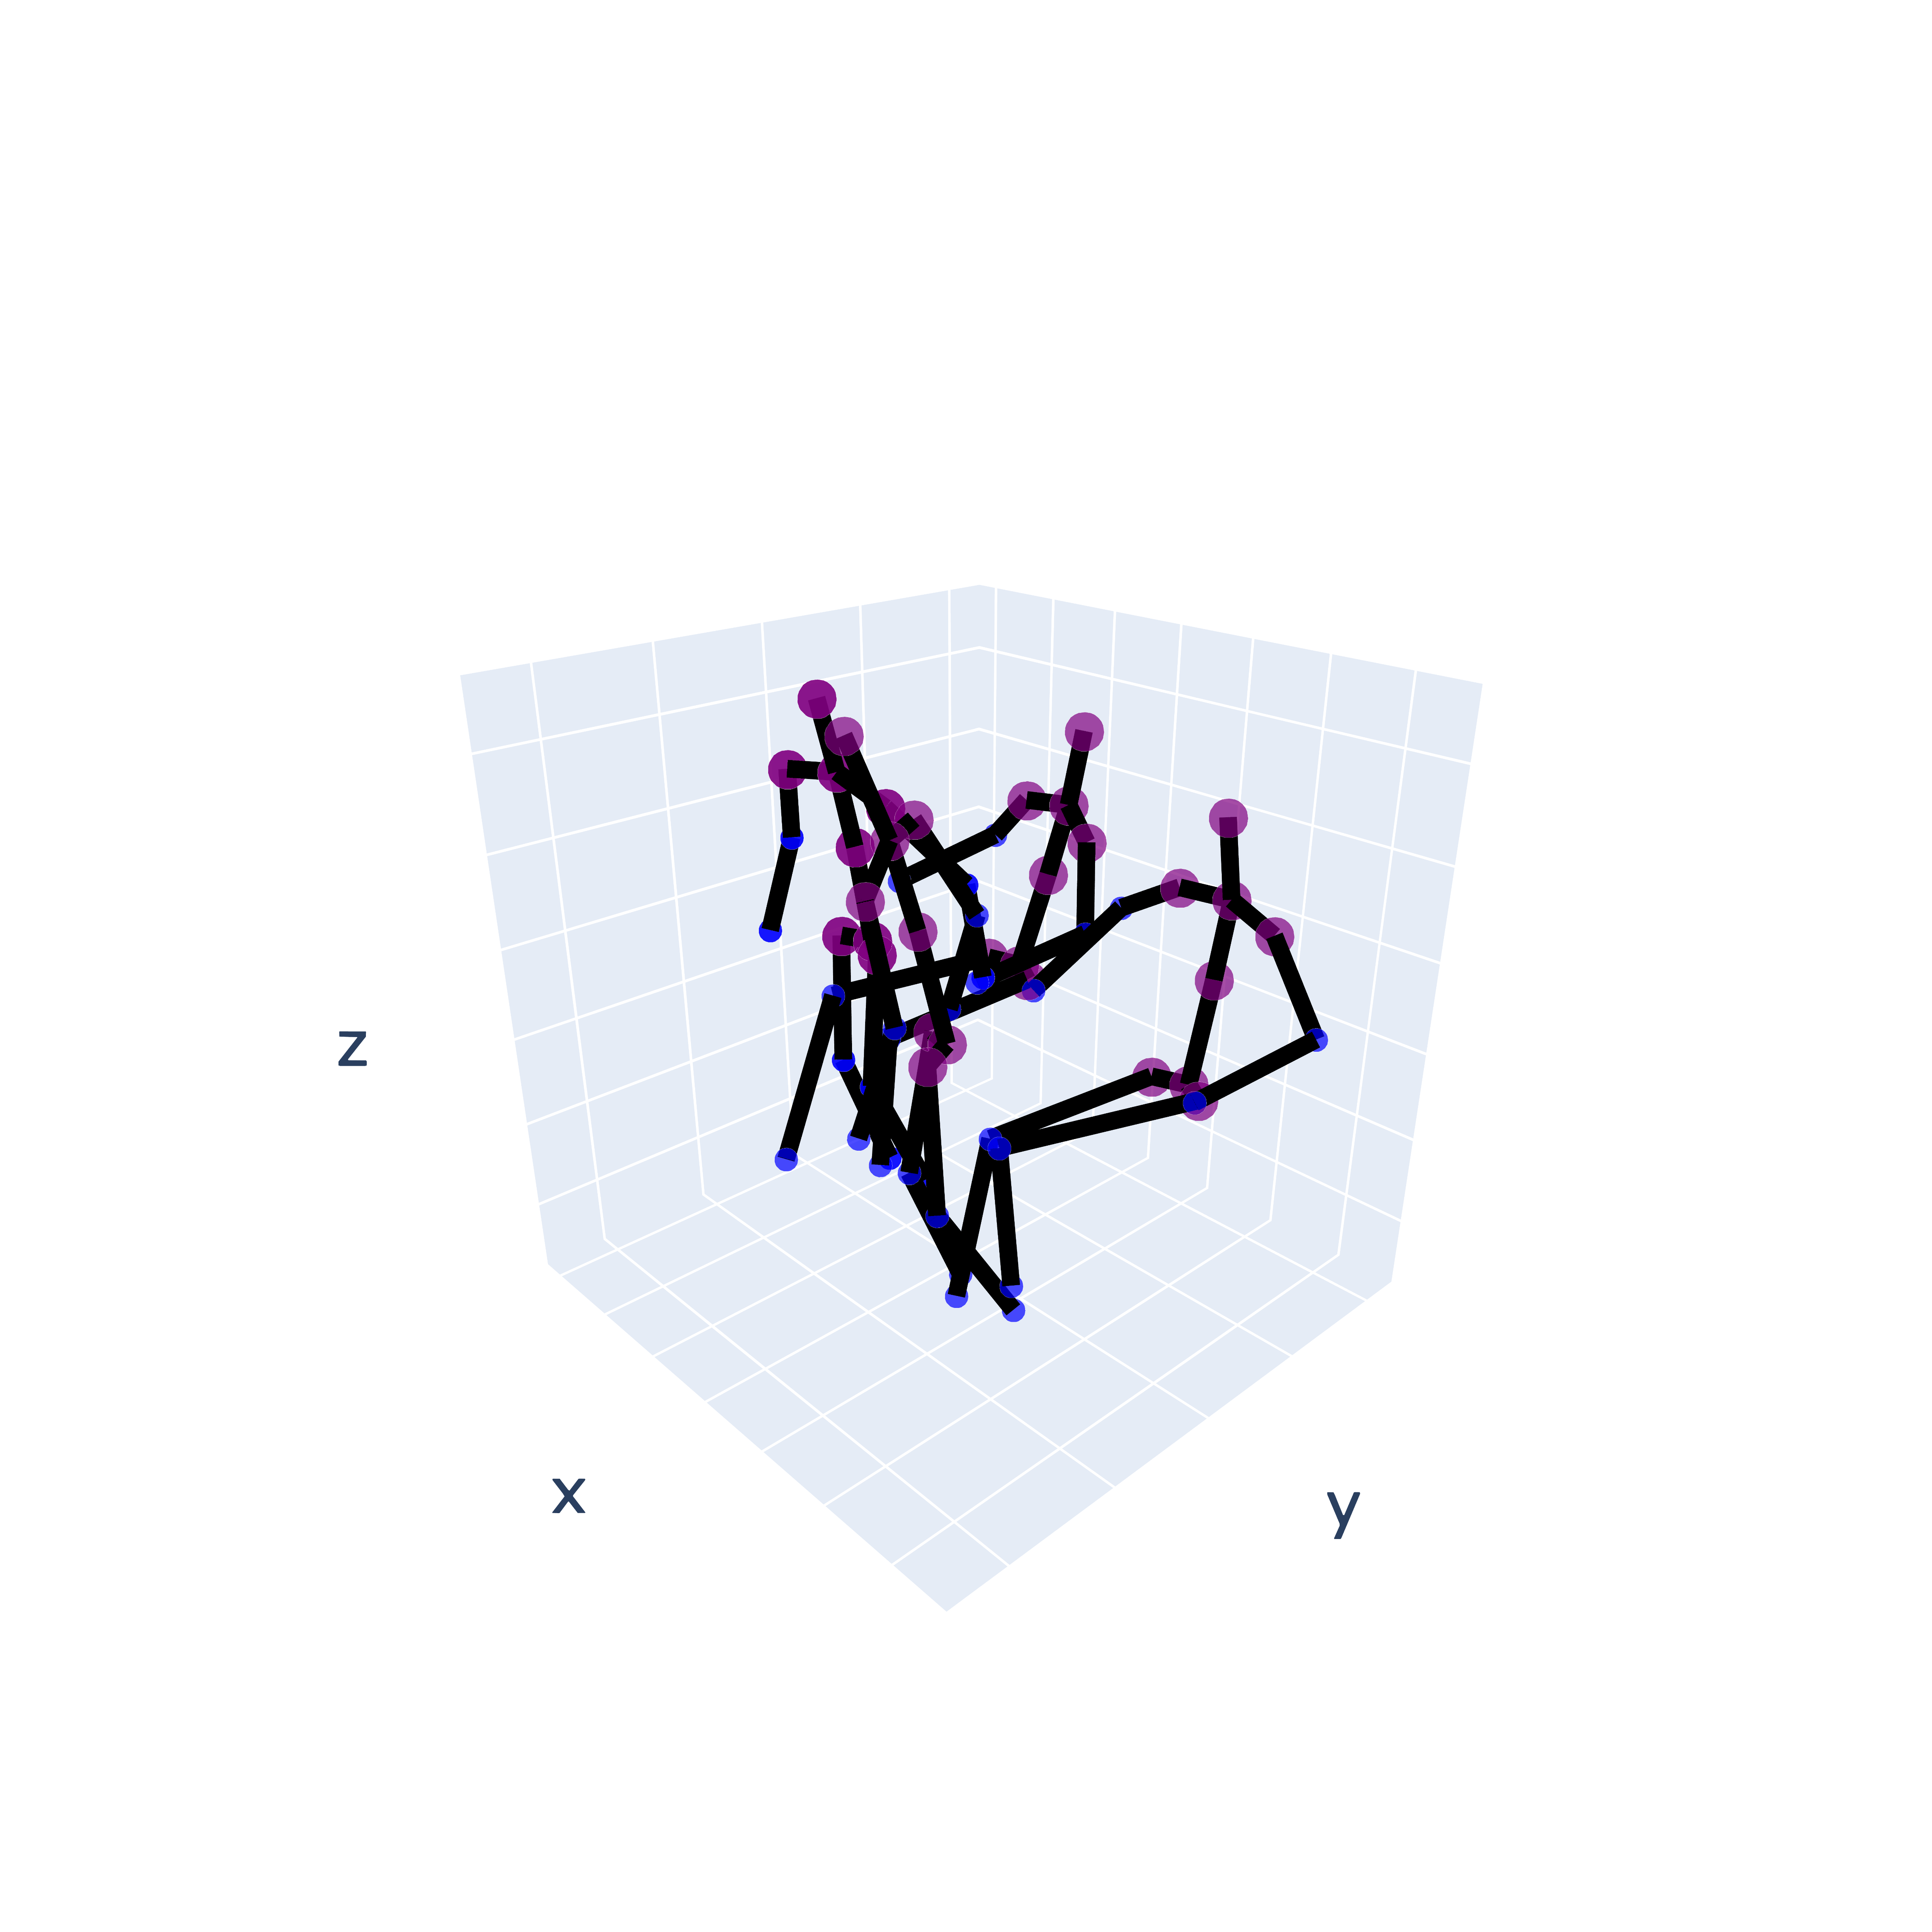
\includegraphics[width=.9\linewidth]{../src/resources/plots/movements/mov-0.png}
                \caption{Chair to Chair}
                \label{fig:mov-0}
            \end{subfigure}
            \begin{subfigure}{.5\textwidth}
                \centering
                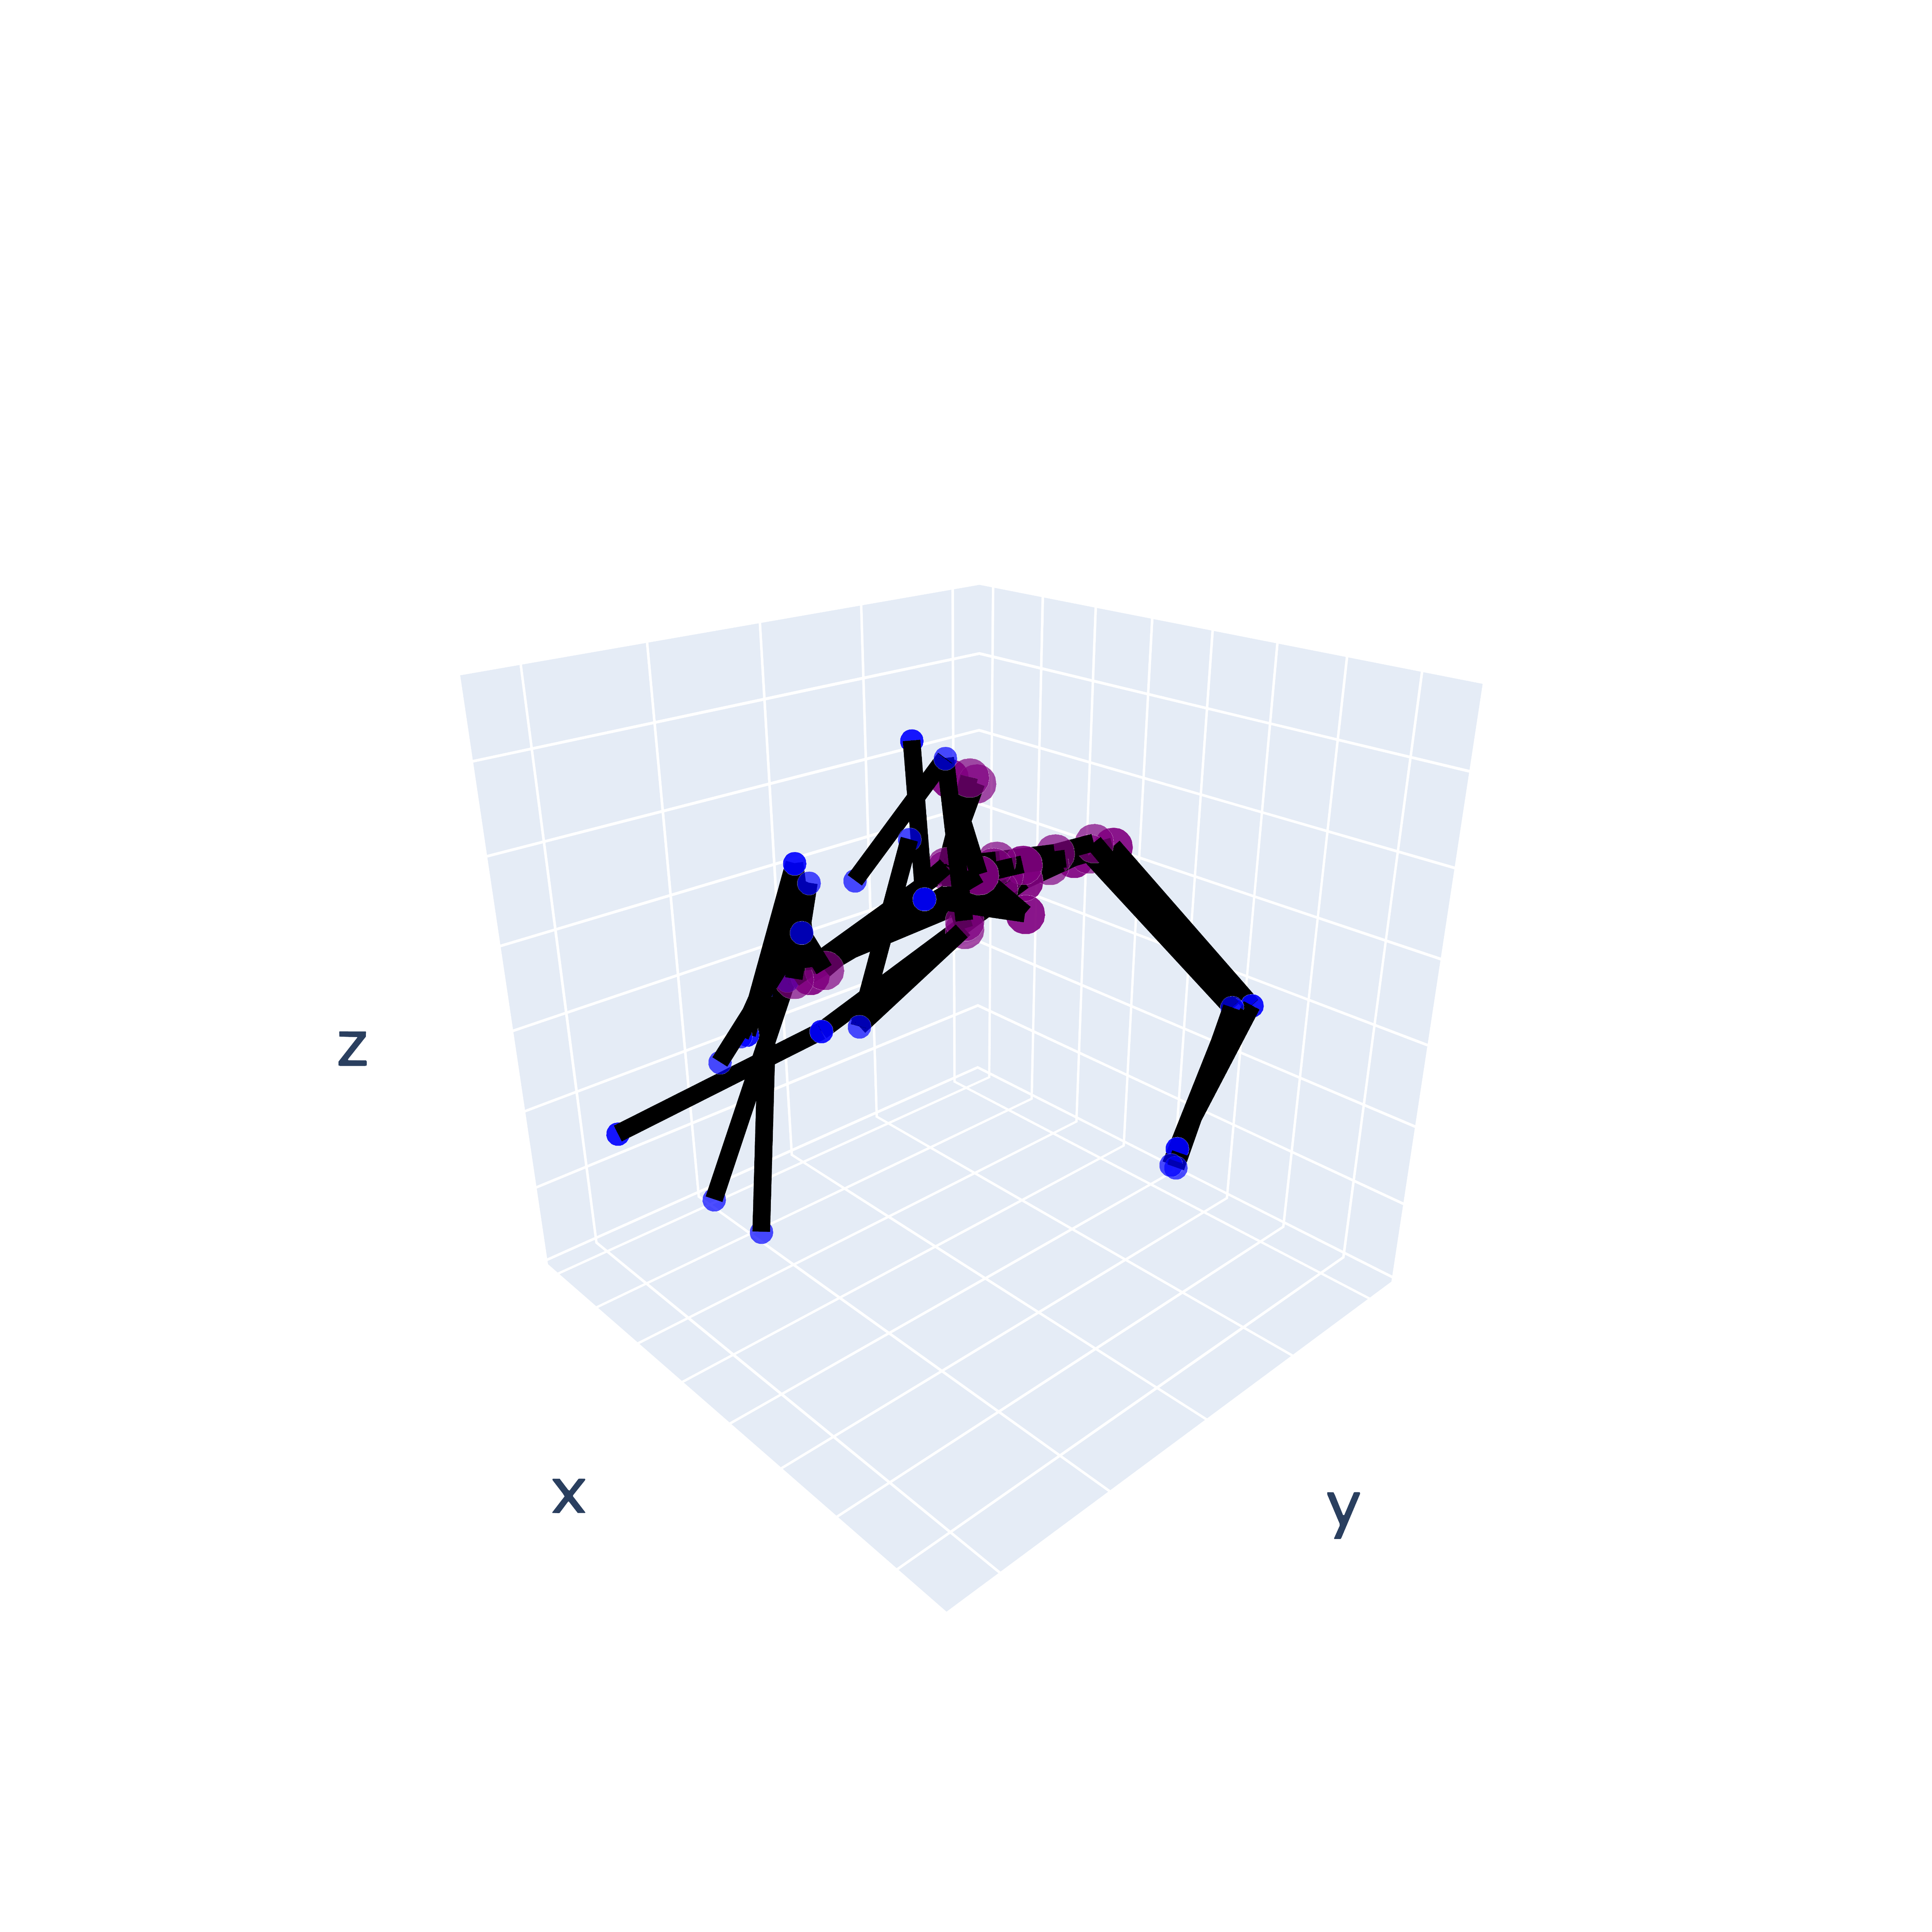
\includegraphics[width=.9\linewidth]{../src/resources/plots/movements/mov-corrupted.png}
                \caption{Chair to Chair corrupted}
                \label{fig:mov-1}
            \end{subfigure}
            
            \begin{subfigure}{.5\textwidth}
                \centering
                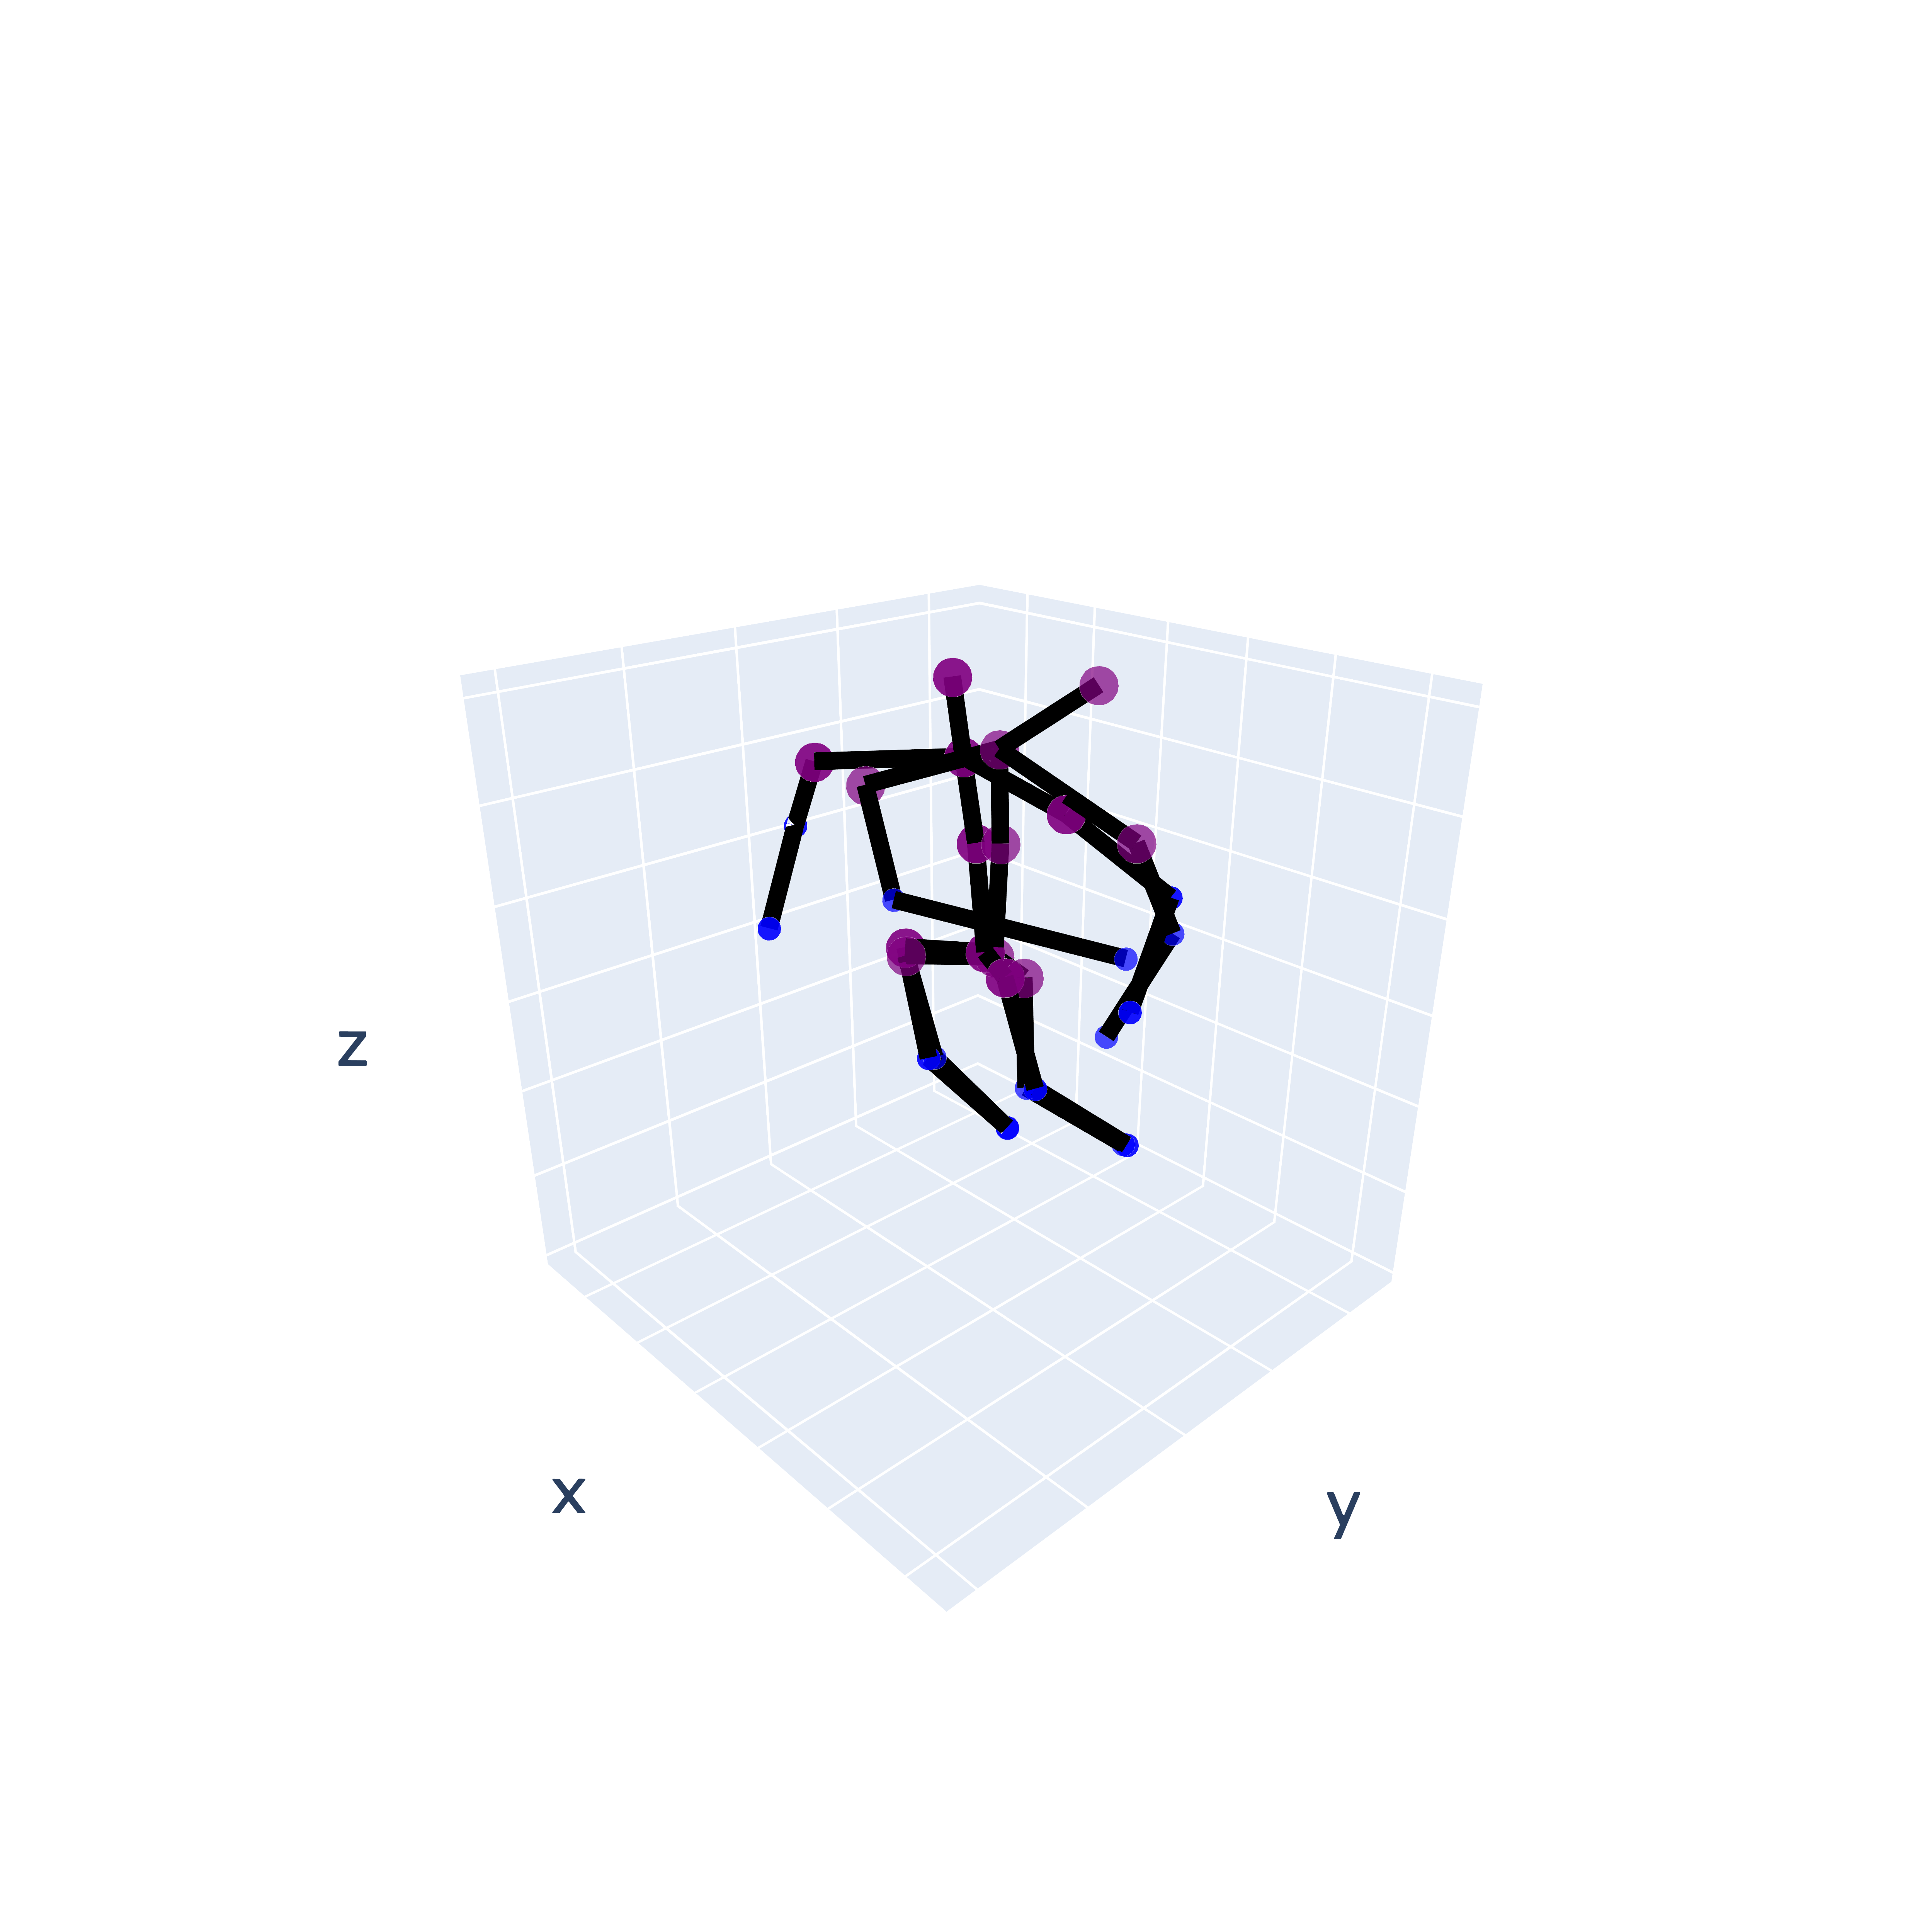
\includegraphics[width=.9\linewidth]{../src/resources/plots/movements/mov-2.png}
                \caption{Cross-Reach Left}
                \label{fig:mov-2}
            \end{subfigure}
            \begin{subfigure}{.5\textwidth}
                \centering
                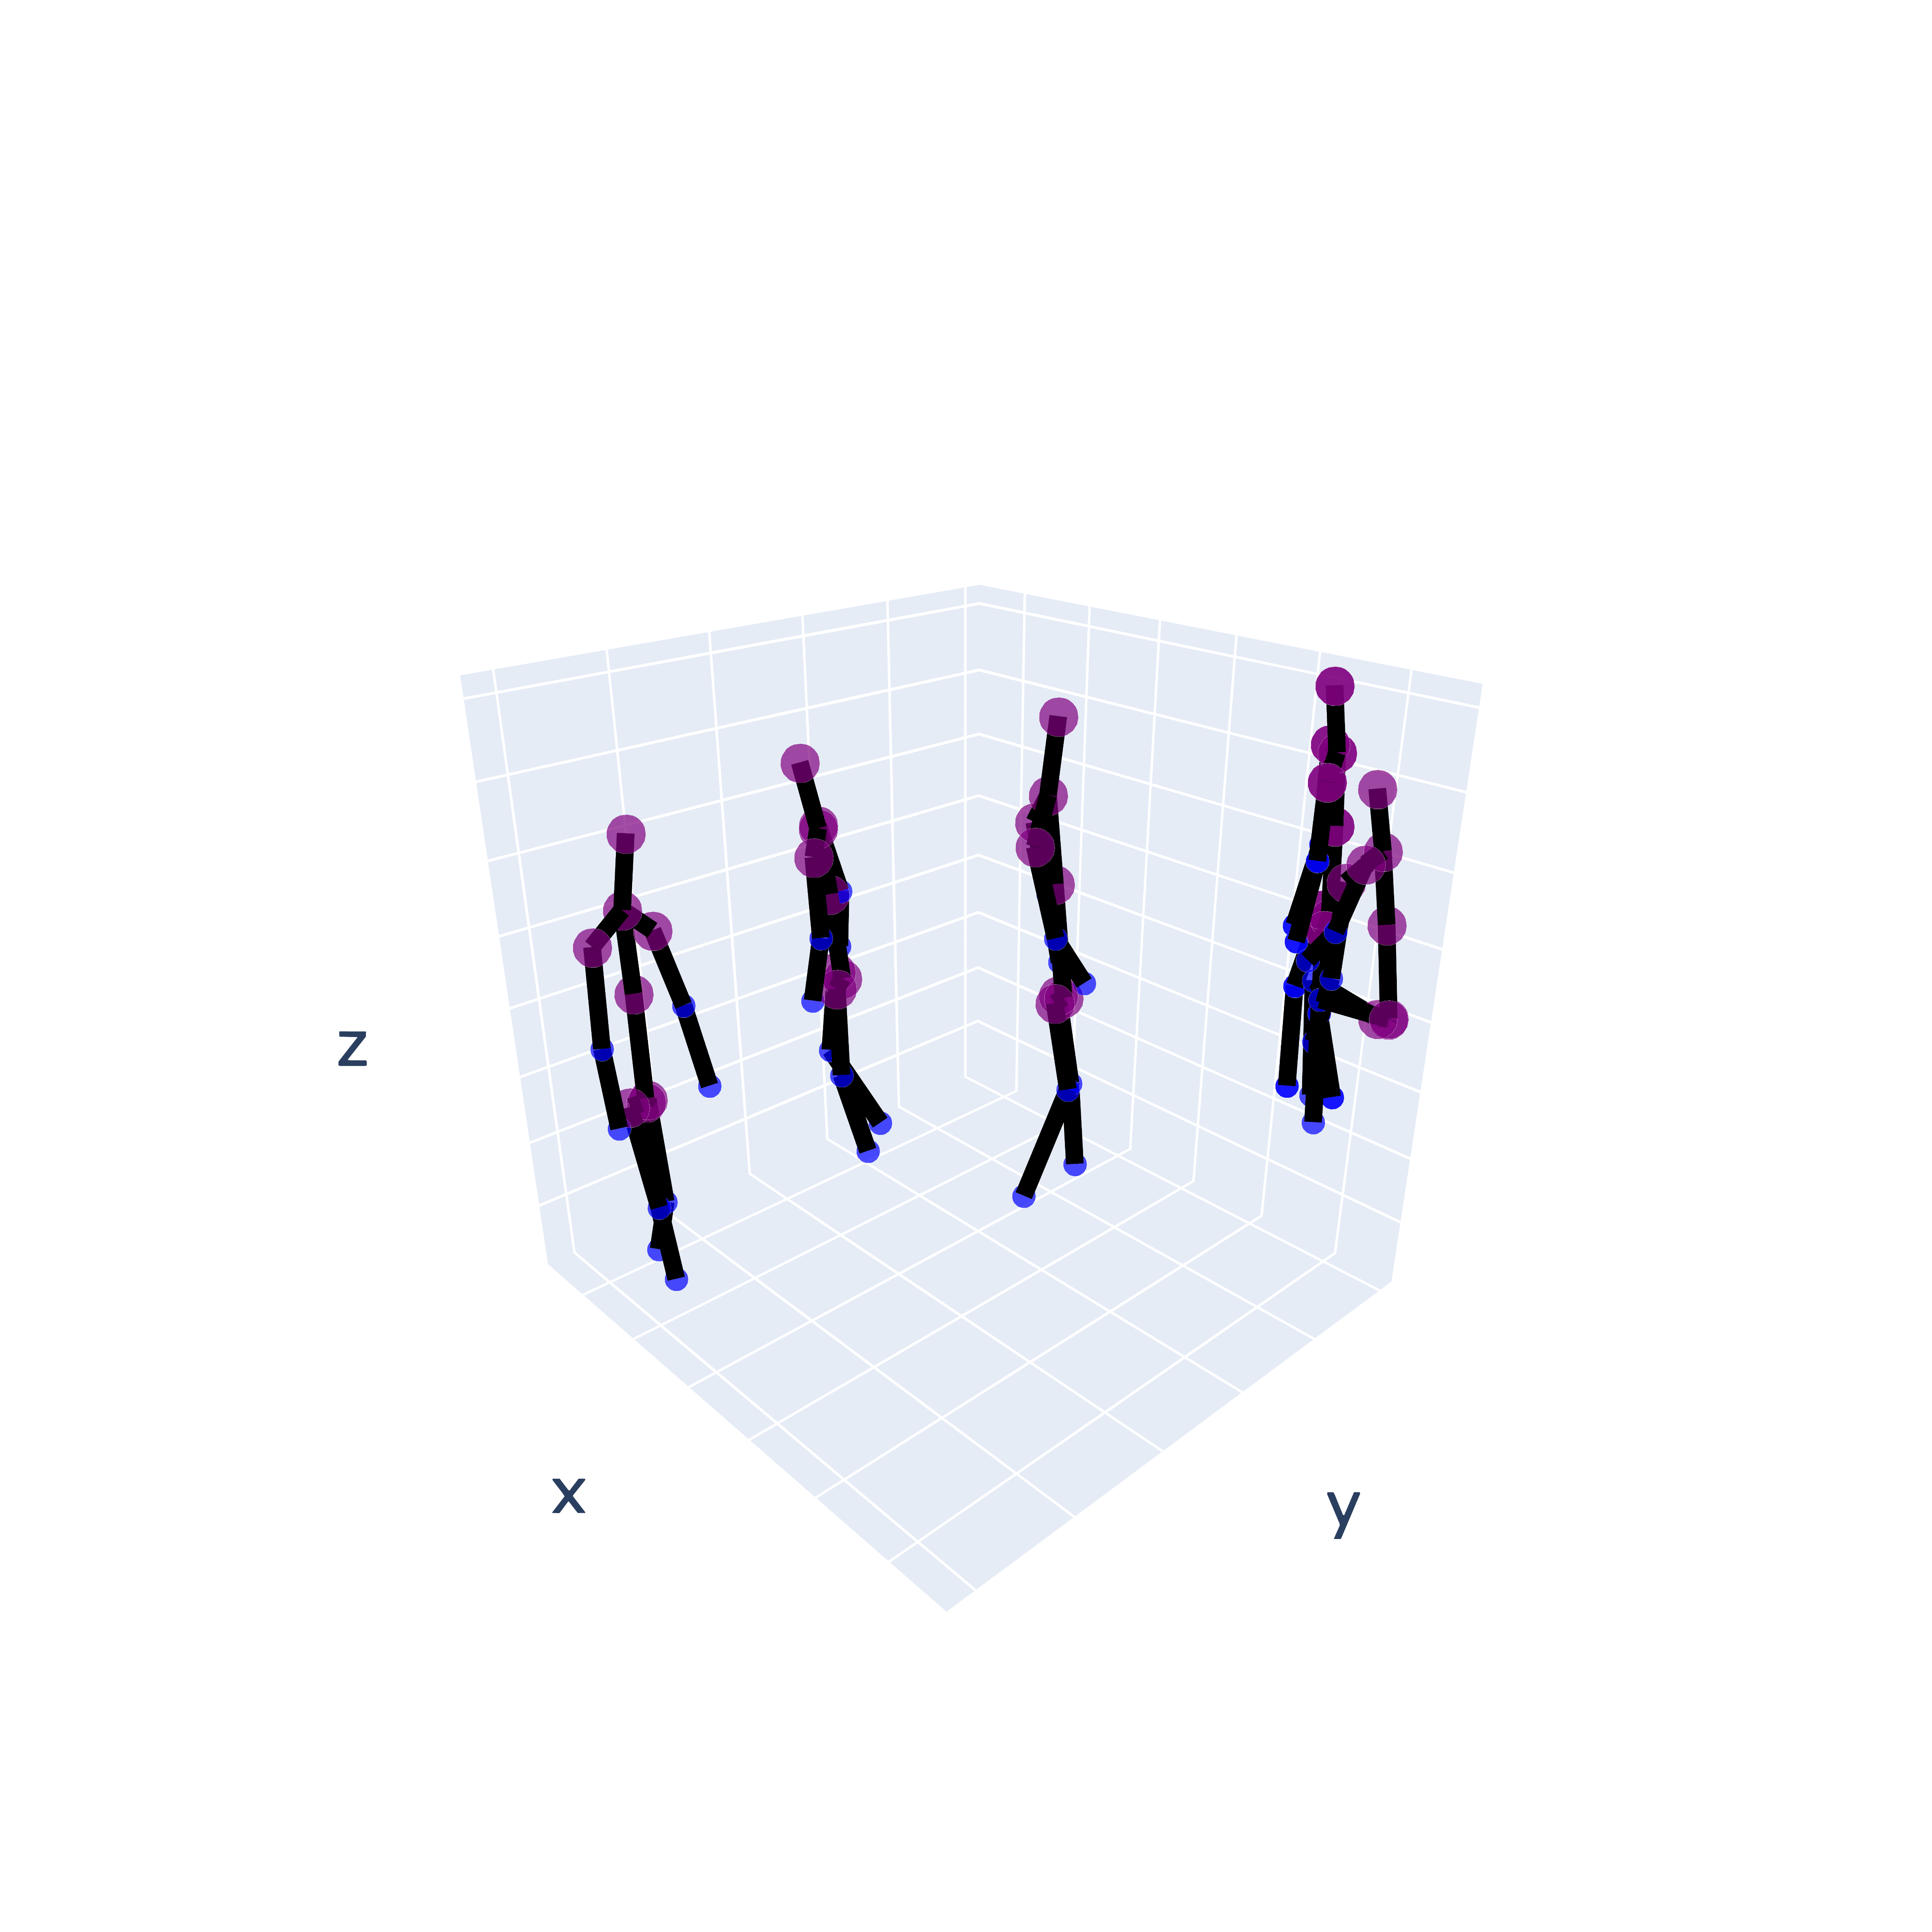
\includegraphics[width=.9\linewidth]{../src/resources/plots/movements/mov-9.png}
                \caption{Tug Walk}
                \label{fig:mov-9}
            \end{subfigure}
            
            \caption{Visualization of movements performed by the patients. Each plot is a 3D visualization containing frames that display the animation.}
            \label{fig:movements_visualization}
        \end{figure}

        Movement visualization allows for the identification of corrupted data, Figure \ref{fig:mov-1} displays a movement that is corrupted, it is not possible to identify the movement due to the data being incorrect. This led to further investigation and the identification of corrupted data in the dataset, all of the data of \textit{Patient-1} is corrupted and is removed from the dataset to not affect the classification task. This corruption is due to the patient not being in the field of view of the Kinect sensor, and the data is not recorded correctly.
        
    \section{Data processing}

        An original dataset containing Kinect skeleton data is processed to remove noise and outliers. This process is needed to improve classification results. Data processing steps are described in the following sections.
        
        \subsection{Cleaning}
        
        From the original dataset, a process of cleaning data is performed. Consisting of removing columns that contain zero values and the ones that are not needed for this classification task. Columns that are kept are listed in Table \ref{tab:joints_select}, only positional coordinates are kept, and state columns and rotation columns (x, y, z) are removed due to not giving any useful information. As mentioned in Section \ref{sec:movements_visualization},  all corrupted data that is identified with the visualization process is removed from the dataset.

        \subsection{Normalization}

        Pose normalization is performed using the formula described in \cite{maudsley-barton_comparative_2017} as follows:
        \begin{equation}
            P_{n,i}(x,y,z) = P_{n,i}(x,y,z)-P_{spinebase,1}(x,y,z)
            \label{eq:pose_normalization}
        \end{equation}

        Equation \ref{eq:pose_normalization} is used to normalize the pose of a patient performing a movement. By subtracting the coordinates of the spine base joint in the first frame from the coordinates of all joints in the data. This is done to remove the effect of the position of a patient in the recording setup and align all frames to the same position. 

        \subsection{Transformation}

        Once data cleaning and normalization are performed, it is transformed into a format that can be used for a classification task. Using the Scikit-Learn library \cite{sklearn_api}, \textbf{MinMaxScaler} is used to scale data between 0 and 1 then \textbf{StandardScaler} is used to standardize it. After this process data is ready for a Machine Learning model.

\cleardoublepage
